\subsection{Introduction}
\subsubsection{Convex set}
Convex set A set $S \subseteq \mathbb{R}^n$ is said to be convex if $\forall 
x,y \in S$, the line segment joining $x$ and $y$ is contained in $S$.

\centerline{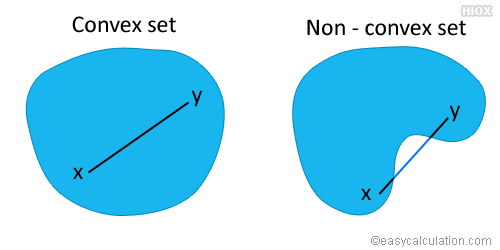
\includegraphics[width=0.5\textwidth]{convex-nonconvex-set.png}}
\subsubsection{Convex Combination}
Given two points $x=(x_1, x_2)$ and $y = (y_1, y_2) \in \mathbb{R}^2$, a convex 
combination of $x$ and $y$ is defined by
\[\lambda x + (1 - \lambda) y = \lambda x_1 + (1 - \lambda)y_1 + \lambda x_2 + 
(1 - \lambda)y_2, \text{ for } \lambda \in [0,1]\]
Changing the value of $\lambda$, we walk thought the segment. In general, 
 is the area confined by the edges formed by points.
 
 \paragraph{Example} Consider a practical example, suppose there are four wells 
$(w_1, w_2, w_3, w_4)$ to generate petroleum and the composition $(A, B, C)$ of 
petroleum from each well are different as follows:

\begin{table}[H]
\centering
\begin{tabular}{|l|l|l|l|l|}
\hline
            &       & A   & B   & C   \\ \hline
$\lambda_1$ & $w_1$ & 0.4 & 0.4 & 0.2 \\ \hline
$\lambda_2$ & $w_2$ & 0.6 & 0.3 & 0.1 \\ \hline
$\lambda_3$ & $w_3$ & 0.3 & 0.4 & 0.3 \\ \hline
$\lambda_4$ & $w_4$ & 0.2 & 0.7 & 0.1 \\ \hline
\end{tabular}
\end{table}
Therefore, all the possible compositions from the mixture of the four kinds of 
petroleum is actually a convex combination of the four petroleum. The four 
wells are like four points in a 3-D space and the convex set is the object 
whose vertices are those four points.

\subsubsection{Convex Hull}
\textbf{Definition 1}: Convex hull of a finite set of points $S$ is the set of 
all points that can be expressed as convex combinations of points in $S$. 

\textbf{Definition 2}: Convex hull of a set of points is the smallest convex 
set that contains these points.
 
More intuitively, convex hull is like a rubber band stretched from infinite and 
struck on the nails on points.
\centerline{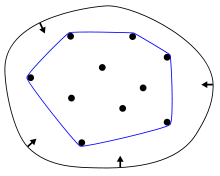
\includegraphics[width=0.5\textwidth]{ConvexHull.png}}
\subsubsection{Convex polygon}
Convex polygon is a polygon which is a convex set. It always contains interior 
angle which smaller than 180 degree.
\subsection{Algorithm}
\begin{itemize}
 \item Input: $n$ points, $(x_1, y_1), (x_2, y_2), \cdots, (x_n, y_n)$.
 \item Output: The sequence of points on the boundary in counter clock order.
\end{itemize}

\subsubsection{Relative Location of Line and Points}
Given a line by two points $(x_1, y_1), (x_2, y_2)$ , a joining segment can 
be represented as follows:
\[y - y_1 = \frac{y_1 - y_2}{x_1 - x_2} (x - x_1)\]

For any third point $(x_3, y_3)$, it is possible determine which side of the 
line the third point lies. For instance, the thirds point is above the segment 
if 
\[y_3 - y_1 > \frac{y_1 - y_2}{x_1 - x_2} (x_3 - x_1)\]

\subsubsection{Convex Hull Successive Points Lemma}
\begin{itemize}
 \item If there is a segment joining two points such that all the other 
points lie on the same side of the segment, the segment represents two points 
on the convex hull.
 \item Conversely, if you have a segment on the convex hull and extending it, 
then every point from the convex hull will lie on the same side of the line.
\end{itemize}

\subsubsection{Baseline}
\begin{enumerate}
\item Use the extreme point as a start $x$.
\item Take every pair of points with $x$. write the equation for the line 
joining them and find the line where all other the points lie on the same side.
\item The line is a segment of convex hull.
\item Set $x$ to the other point of the segment and then repeat step 2.
\end{enumerate}

\paragraph{Runing Time Analysis}
\begin{itemize}
\item Determine all the points are on the same side of segment takes $O(n)$ 
steps.
\item To find one convex hull segment, we should check $O(n)$ segments.
\item There are at most $O(n)$ convex hull segment.
\item Therefore, the total run time is $O(n^3)$.
\end{itemize}

\subsubsection{Merge Hull}
Tips: To be efficient, we could like the sizes of sub-problems in divide and 
conquer to be same.
\begin{enumerate}
 \item Divide points into those with $x$-coordinates $\le x_{median}$ and those 
with $x$-coordinates $> x_{mdian}$.
\item Recursively find the convex hull for the points on the left and right.
\item Find the upper tangent and lower tangent of the two convex hull. 
\item Start from the left of upper tangent and walk through the left convex 
hull counterclockwise until meet the lower tangent. Then move to the right 
convex hull and keep walking until back to the upper tangent.
\end{enumerate}
\centerline{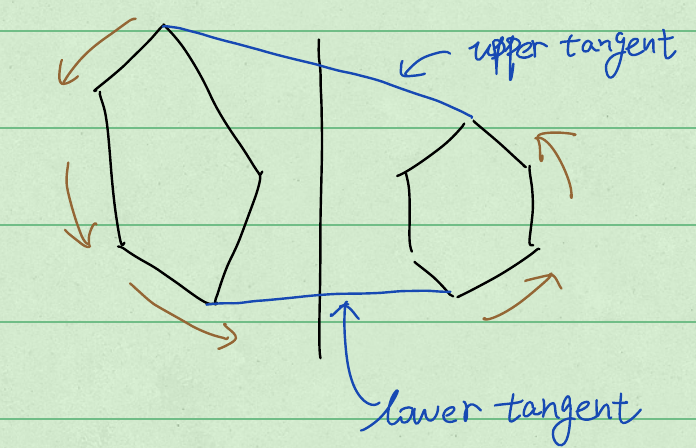
\includegraphics[width=0.5\textwidth]{tangent.png}}

\paragraph{Remarks:}
\begin{itemize}
\item Points on one hull can ``\textbf{see}'' a point on the other hull if the 
segment joining the two points does not intersect either hull.
\item Upper tangent, lower tangent are pairs of points that see each other.
\item \textbf{Upper tangent}  is the highest line segment joining two vertices, 
one from each hull, that see each other.
\item Similar with the lower tangent. Therefore the total running time is 
$O(n)$.
\end{itemize}

\paragraph{Stab}
A line $pq$ stabs to $C_2$ if the continuation of the line goes to 
the interior of $C_2$.

\paragraph{How to check stabbing}
\begin{itemize}
\item If the segment $pq$ stabs $C_2$, then the clockwise predecessor of $q$ 
is on the one side of the segment and the clockwise successor of $q$ is one the 
other side.
\item If $pq$ stabs $C_2$ then $p$ must be able to see the clockwise 
predecessor and successor of $q$.
\end{itemize}

\paragraph{How to find the upper tangent:}
The upper tangent can be found by a ``swirling'' algorithm.
\begin{itemize}
\item Choose $p$ to be the right most point in the left hull ($C_1$) and 
$q$ to be the left most point in the right hull ($C_2$). Then $p$ and $q$ see 
each other. 
\item If $pq$ stabs to $C_1$, move $p$ to its counterclockwise successor.
\item If $pq$ stabs to $C_2$, move $q$ to its clockwise successor.
\item repeat until $pq$ does not stab to any hull. Then $pq$ is the upper 
tangent.
\end{itemize}

Lower tangent can be find with the similar strategy.

\paragraph{Running Time Analysis}
We never repeat the same pair of vertices since once you decide to abandoned a 
vertex in searching of upper tangent, you never come back to it. It means at 
most $n$ vertices to find the upper tangent.

Similarly for the lower tanget.

\subsubsection{Quick Hull}
Like QuickSort, Quick Hull does not have worst case analysis.
\begin{itemize}
\item Pick the left most point $p$ and right most point $q$ on the convex hull 
and draw a segment joining them.
\item Recursively find the convex hull for each side of the points. Each hull 
must contains the segment $pq$.
\item Merge the two hull by glue them on segmeng $pq$.
\end{itemize}

We did not spend too much time on how to find the next two pair of points at 
each iteration. But here are some remarks.

\paragraph{Remarks}
\begin{itemize}
 \item Always pick points on $x$ direction my casue the worst case, which is 
all the points are aggregated to one side of line.
\item Like quicksort, introducing randomness helps achieve the optimal average 
running time. We randomly choose a direction and project all the points on it. 
Pick the two extremes as the points for the next iteration.
\end{itemize}